\chapter{Transport Protocols}
\section{UDP -- User Datagram Protocol}
\begin{itemize}[nosep]
    \item Unreliable, unordered datagram service
    \item Adds multiplexing checksum
    \item End points identified by \emph{ports}
          \begin{itemize}[nosep]
              \item Scope is an IP address (interface)
          \end{itemize}
    \item Checksum aids in error detection
\end{itemize}
\url{https://en.wikipedia.org/wiki/User_Datagram_Protocol}
\subsection{UDP Header}
\begin{figure}[H]
    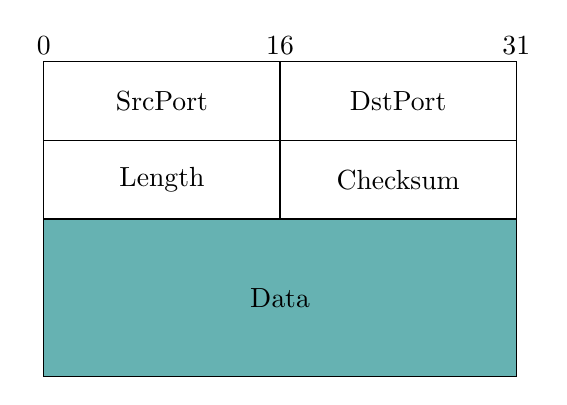
\begin{tikzpicture}
        \draw (0, 0) rectangle (3, -1);
        \draw (0, -1) rectangle (3, -2);
        \draw (3, 0) rectangle (6, -1);
        \draw (3, -1) rectangle (6, -2);
        \draw[fill=teal!60!white] (0, -2) rectangle (6, -4);

        \node at (1.5, -0.5) {SrcPort};
        \node at (4.5, -0.5) {DstPort};
        \node at (1.5, -1.5) {Length};
        \node at (4.5, -1.5) {Checksum};
        \node at (3, -3) {Data};

        \node at (0, 0.2) {0};
        \node at (3, 0.2) {16};
        \node at (6, 0.2) {31};
    \end{tikzpicture}
\end{figure}